\documentclass[11pt, oneside]{article}   	% use "amsart" instead of "article" for AMSLaTeX format
\usepackage{geometry}                		% See geometry.pdf to learn the layout options. There are lots.
\geometry{letterpaper}                   		% ... or a4paper or a5paper or ... 
%\geometry{landscape}                		% Activate for rotated page geometry
%\usepackage[parfill]{parskip}    		% Activate to begin paragraphs with an empty line rather than an indent
\usepackage{graphicx}				% Use pdf, png, jpg, or eps§ with pdflatex; use eps in DVI mode
								% TeX will automatically convert eps --> pdf in pdflatex		
\usepackage{amssymb}

%SetFonts
\graphicspath{ {./images/} }

%SetFonts


\title{Sicurezza e Privatezza}
\author{Federico Zhou}
%\date{}							% Activate to display a given date or no date

\begin{document}
\maketitle
%\section{}
%\subsection{}
Ore: 3 ore Lunedì, 2 il Mercoledì\\
4,5 crediti di teoria 1,5 di laboratorio\\\\
Computer security refers to measures and controls that ensure confidentiality, integrity and availability of information system assets including hardware, software, firmware and information.\\
\begin{itemize}
\item Confidentiality: is the avoidance of the unauthorized disclosure of information
\item Integrity: the information cannot be altered in an unauthorized way\\
Proprietà che garantisce la preservazione da modifiche non autorizzate
\item Availability: ensuring timely and reliable access to and use
\item Accountability: to ensure the non repudiability, aided by log files
\end{itemize}
Le misure di cybersecurity da adottare sono in proporzione al livello di impatto che una potenziale intrusione può causare. I livelli di impatto possono essere basso, medio (serious adverse effect on organizational operations) o alto (una perdita che causa problemi catastrofici to the organizational operations, assets or individuals).\\
\emph{Brutalmente: alloco una quantità di effort in proporzione al danno che un potenziale fallimento può portare: polizza bicicletta $\neq$ polizza auto}\\\\
Keywords:\\
\textbf{Security policy:} set of criteria for the provision of security services. Una collezione di scelte adottate per definire le condizioni per la sicurezza informatica\\
\textbf{L'asset:} l'oggetto che deve essere protetto, comprende tutto il patrimonio informativo fisico di di un gruppo di sistemi\\
\textbf{Threat:} circostanze o eventi che possono impattare in maniera negativa le operazioni\\
\textbf{Vulnerability:} debolezza presente in un sistema\\\\
\section*{Introduzione alla crittografia}
La crittografia ha come obbiettivo fornire \textbf{confidenzialità} ai dati trasmessi o memorizzati. La crittografia è suddivisa simmetrica o asimmetrica qualora vi siano rispettivamente una o due chiavi (la chiave per cifrare è la stessa per decifrare, o più). E' fondamentale che le chiavi crittografiche siano private e accessibili solo dal mittente e dal destinatario.\\
Attraverso \emph{l'attacco via cryptoanalisi}, l'attaccante analizza la natura degli algoritmi, e cerca di ricavarne informazioni al riguardo; un'altro tipo di attacco è quella per \emph{brute-force}.\\
La sicurezza di un algoritmo di crittografia dipende dalla sua resilienza ai tentativi di decrittaggio; ne consegue che un algoritmo pubblico che rimane resistente dopo anni è più resiliente di un algoritmo privato (più persone ci sono che cercano di bucarlo, più resiliente diventa). \\\\I principali algoritmi simmetrici sono \emph{DES, Triple DES, AES}. Questi algoritmi funzionano frammentando il plaintext in blocchi di grandezza uguale (64 bits per DES, 128 per AES), e restituendo un cyphertext di grandezza medesima; cambia invece la grandezza della chiave (56 per DES, 112 o 168 per Triple DES, 192 o 256 per AES).\\
Il DES (o Data Encryption Algorithm) è basato su blocchi di plaintext di 64 bit, crittografati con una chiave di 56 bit per produrre un cyphertext di 64 bit.\\
Il Triplo DES (o 3DES) è basato sul DES, e ripete le operazioni algoritmiche del DES 3 volte, utilizzando due o 3 chiavi univoche.\\
L'AES (Advanced Encryption System) (precedentemente chiamato Rijndael) \\\\
L'electronic codebook (ECB) è la modalità più pratica per approcciare la decrittaggio, dividendo il cyphertext in più blocchi abilitando la parallelizzazione. 
\begin{center}
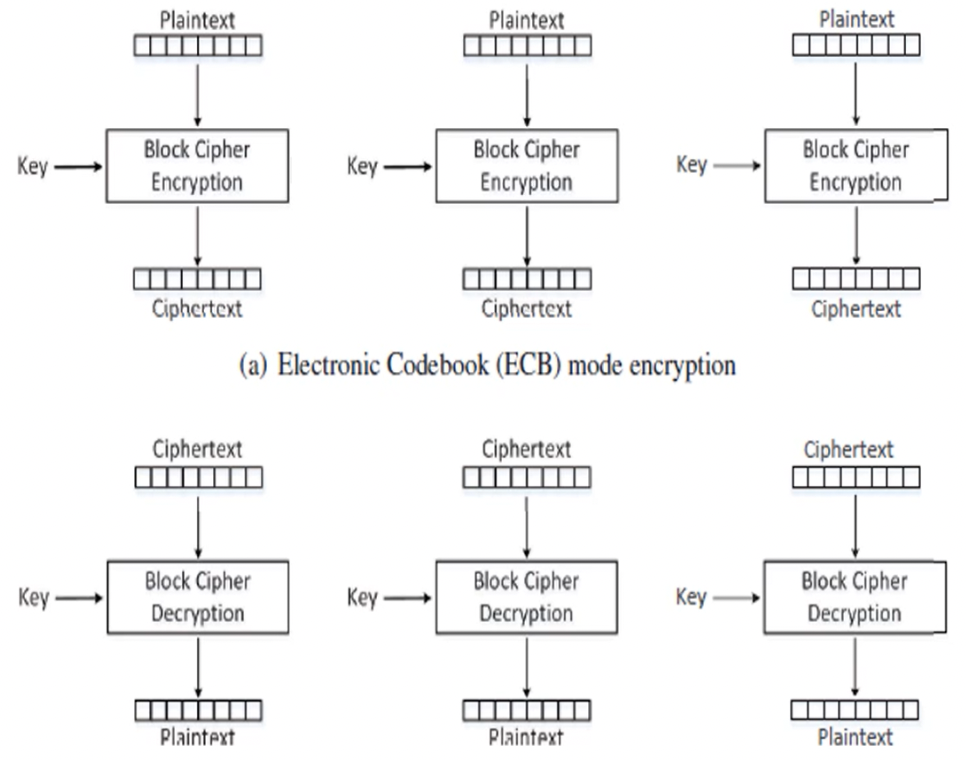
\includegraphics[scale=0.5]{ECB}
\end{center}
Il Cypher Block Chaining (CBC) consiste nel combinare in XOR (genera più casualità) utilizzando l'output del processo di crittografia precedente come input per il prossimo.
\begin{center}
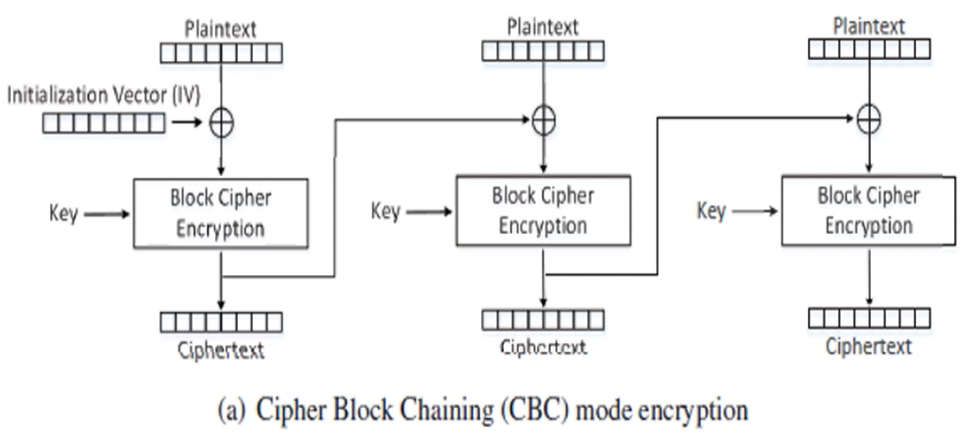
\includegraphics[scale=0.5]{CBC}
\end{center}
Block cypher vs Stream cypher \\
Il block cypher processa in input un blocco alla volta, può riutilizzare le chiavi ed è più comune; mentre lo stream cypher processa elementi in input in maniera continua, processa gli elementi uno alla volta.\\\\
La crittografia, se ben utilizzata, ci fornisce uno strumento resiliente per garantire la \textbf{confidenzialità}, ma possiamo garantire anche che il messaggio non sia stato alterato \textbf{(integrità)}, per verificare che il messaggio sia effettivamente inviato da chi dice id averlo inviato \textbf{(autenticità)}, e la verifica di appartenenza \textbf{(autenticità)}\\
Un modo di garantire l'autenticità e l'integrità è attraverso il MAC, ovvero il \emph{Message Authentication utilizzando un Message Authentication Code}. Il ricevente verifica l'integrità del dato, che viene fatto integrando al messaggio un tag (a sua volta cifrato), condiviso tra mittente e destinatario.\\
Hashing function: SHA and md5\\\\
\emph{Diffie-Hellman attack}
Come può Bob fidarsi del fatto che un messaggio che ha ricevuto appartiene effettivamente ad Alice? Per ovviare a questo problema è stato introdotto un meccanismo di verifica, Bob, per fidarsi, verifica che il messaggio sia segnato con un certificato di autenticità emesso da un'autorità, o da una terza parte fidata.\\\emph{Public key certificates | GPG}\\
I meccanismi di attestazione di validità di public key sono: GPG e PKI. L'idea di base è quella di associare un certificato alla chiave pubblica; ovviamente il certificato deve essere non modificabile, emesso dalla certification authority
\begin{center}
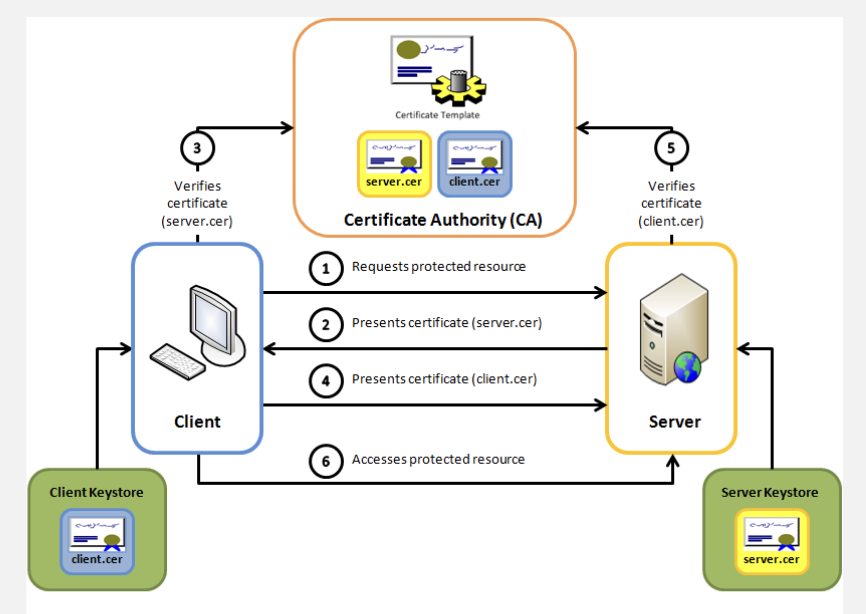
\includegraphics[scale=0.7]{asd}
\end{center}
Questo meccanismo è utilizzato anche per verificare le transazioni con carte basate su Visa e Mastercard. GPG è anche utilizzato per verificare la validità del software, viene generato un file .hmac, che viene verificato con la chiave pubblica. A livello internazionale, le chiavi pubbliche sono salvate all'interno di un server pubblico chiamato key ring.\\\\
L'autenticazione dell'utente\\
Prima di iniziare andiamo a distinguere la differenza tra l'identificazione e l'autenticazione. Attraverso l'identificazione dichiariamo di essere un dato soggetto, e attraverso l'autenticazione confermiamo di essere effettivamente tale soggetto.\\\\
Per l'autenticazione abbiamo principalmente 4 strategie:\\
- attraverso un segreto condiviso: passwords e PIN\\
- attraverso il possesso di un particolare token: smartcard, bancomat etc.\\
- attraverso qualità biometriche delll'utente: impronte, retine, faccia etc.\\
- attraverso comportamenti biometrici dell'utente: voce, scrittura etc.\\
Per potenziare ulteriormente è possibile introdurre il 2-factor-authentication in cui vengono combinate 2 modalità di autenticazione.\\\\
Quando parliamo \emph{dell'assurance level} parliamo del livello di confidenza che vogliamo instaurare rispetto ad un meccanismo di autenticazione. E' una scala crescente, che passa va dal livello 1, in cui vi è poca, o nessun livello di confidenza (no password etc) fino al livelo 4, in cui vi è un alto livello di sicurezza.\\
Il \emph{potential impact} va a definire i 3 livelli di impatto su organizzazioni o persone che andrebbero ad intaccare nel caso di una breccia di sicurezza. L'impatto può essere basso, medio o alto.\\\\
\emph{Password-Based Authentication}\\
Il meccanismo più diffuso, l'utente fornisce un nome/logic e password, che viene confrontato col valore che il sistema detiene; in base al tipo di utente sono garantite le autorizzazioni.\\
 Le password sono salvate sul sistema in maniera cifrata, per garantire la confidenzialità anche rispetto al system manager. \\Nei sistemi moderni la password è combinata al \emph{salt} (una chiave), l'unione della quale è passata all'interno di una hash function, valore cui output è salvata all'interno del \emph{password file}.\\
 Al momento dell'autenticazione è recuperato il salt e la hashed password; il salt e la password sono ripassate all'interno della hash-function, output che è comparato con la hashed password.
 \begin{center}
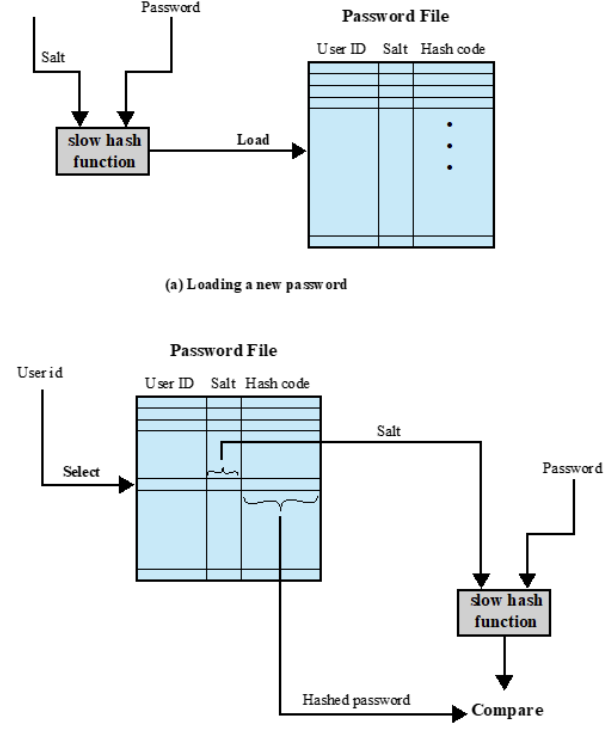
\includegraphics[scale=0.7]{salt}
\end{center}
La hash function deve essere "slow", per prevenire il brute-forcing. In UNIX l'hashing function era il DES ripetute 25 volte, che tuttavia risulta sorpassato. Altri algoritmi di hashing che sono utilizzati sono l'MD5 e Blowfish. In UNIX le informazioni riguardo all'utente sono salvate all'interno il file \emph{passwd}, il file \emph{shadow} che contiene le password hashate.\\ \\
I metodi di attacco per le password sono:
\begin{itemize}
\item Social engineering: un attaccante ottiene la password di un altro utente, alcuni esempi possono essere lo \emph{shoulder surfing o phishing}.
\item Password cracking: \\
- Dictionary attack: confrontando le password con dei dizionari precompilati che contengono le password più diffuse. Ogni file deve essere combinata al salt e hashata per effettuare un confronto.\\
\emph{elenco di password in chiaro, che vengono hashate al momento del confronto}\\
- Rainbow table attacks: computa in anticipo i valori di confronto per tutti i salts possibili, per poi confrontarle. Più il salt è grande più difficile sarà attaccarlo.\\
\emph{elenco di password già hashate per \emph{n salt}, che vengono poi confrontate}\\

 \emph{John the Ripper} è un open-source password cracker sviluppato nel 1996 che utilizza una combinazione di brute-force e dictionary attack.\\
 \end{itemize}
 Gli \textbf{smart token} solitamente possono contenere microprocessori integrati, sono dispositivi che quanod messi a contatto con dispositivi elettronici permettono l'autenticazione. Lo smart token più importanti sono le carte di credito/bancarie. \\
 \textbf{L'autenticazione biometrica} utilizza caratteristiche fisiche (impronte, iride, faccia etc.) di un utente, è basta sul riconoscimento di pattern, è più sicuro delle password, ma è più costosa. Le caratteristiche sono digitalizzate e salvate su un database biometrico.\\
 
L'access control si occupa di prevenire l'accesso e l'utilizzo non autorizzato di una risorsa.
Per scaglionare gli accessi è quindi necessario definire una security policy.\\
Il meccanismo di accesso da parte di un utente avviene un una serie di fasi ben definite:
\begin{itemize}
\item L'utente, attraverso una funzione di autenticazione effettua l'autenticazione
\item L'utente autenticato è usato come input per una funzione di access control\\
L'access control function è definita all'interno di una \emph{authorization database}, definita dal \emph{security administrator}.
\item Se l'utente autenticato ha permessi definiti nell'access control sufficientemente alti ha accesso alle risorse del sistema, altrimenti è respinto.
\end{itemize}
Per verificare a posteriori che gli accessi siano stati forniti in maniera corretta, viene effettuato il processo di auditing basato su logs.
I 3 meccanismi su cui si basa la sicurezza vanno a formare "the gold standard" (dato che iniziano tutti con \emph{AU} ovvero \emph{Autheticazion process, Authorizing access e Auditing} .
 
Quali sono gli attori in un meccanismo di controllo di accesso?
\begin{itemize}
\item I soggetti: sono le entità attive, in grado di accedere ad oggetti, possono essere i proprietari, gruppi, o il resto del mondo
\item Gli oggetti: sono elementi passivi, rappresentano le risorse a cui l'accesso è controllato
\item Access right: descrivono i tipi di operazioni in cui un soggetto può accedere ad un oggetto
\end{itemize}
Access control policies:
\begin{itemize}
\item Discretionary access control (DAC)\\
Gli accessi sono regolamentati in base all'identità del richiedente e alle regole di accesso.
In questo schema i permessi di accesso sono gestiti da parte di un owner attraverso una matrice di accesso (o access control matrix). Queste access control matrix sono salvati all'interno dei metadati dei file, all'interno degli i-node.
 \begin{center}
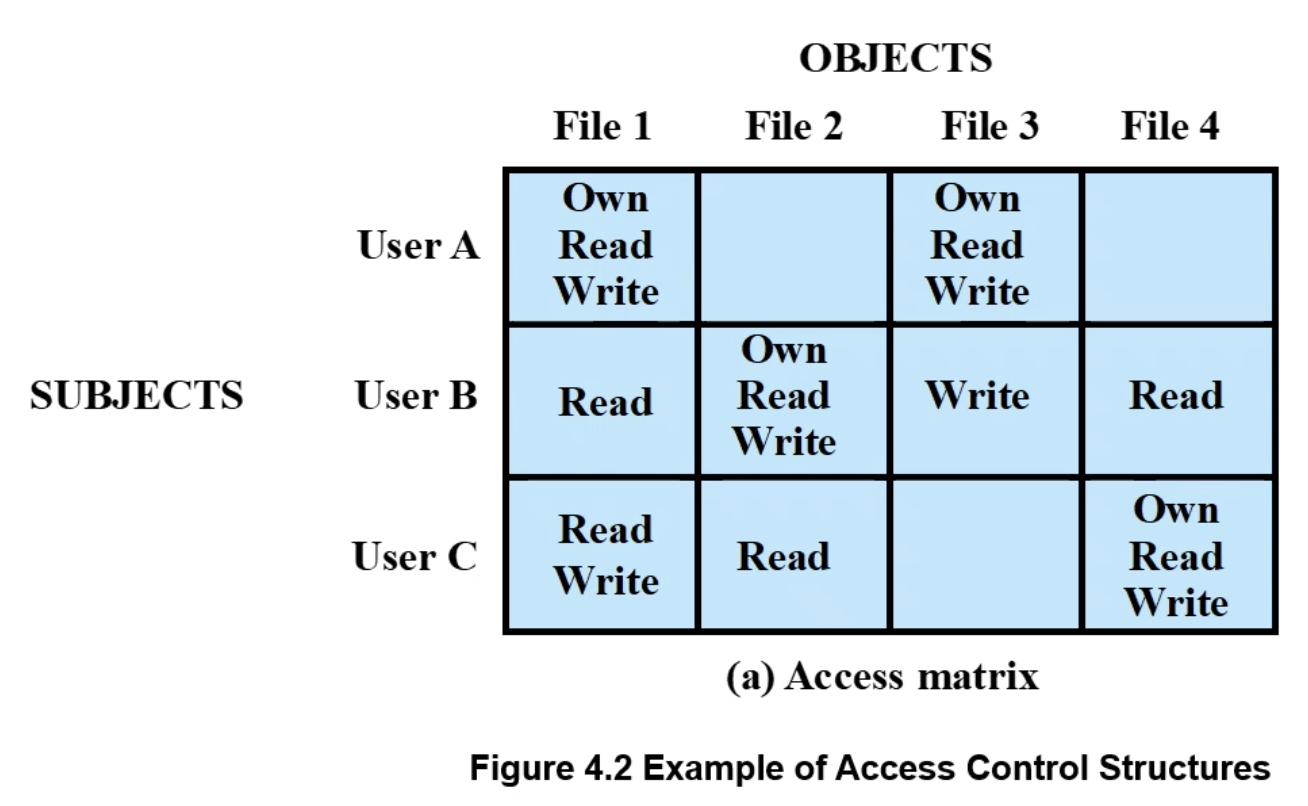
\includegraphics[scale=0.5]{mac}
\end{center}
\emph{Il problema di questa matrice è il grosso spreco di spazio, e la prevalenza di caselle vuote}\\
Un'alternativa a questa soluzione è la access control list.
 \begin{center}
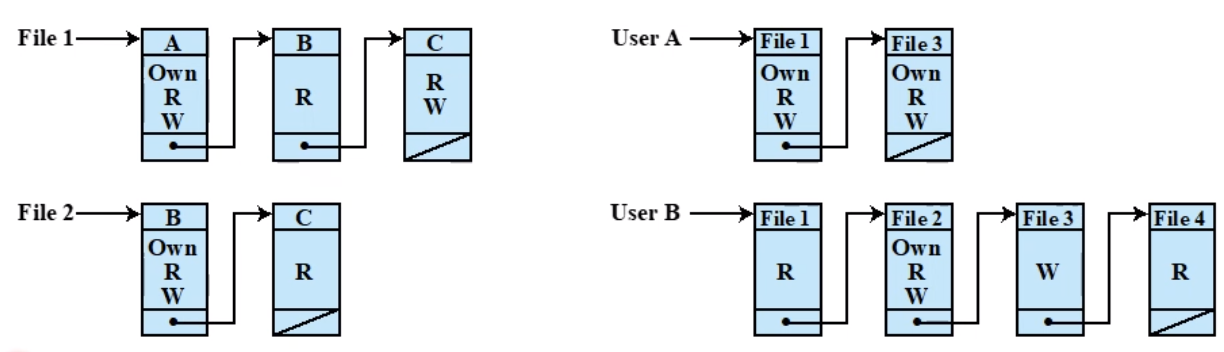
\includegraphics[scale=0.5]{acl}
\end{center}
Quando un utente B vuole accedere al file 2, vengono controllati i metadati del file, e qualora sia abilitato, l'accesso sarà concesso.
\begin{center}
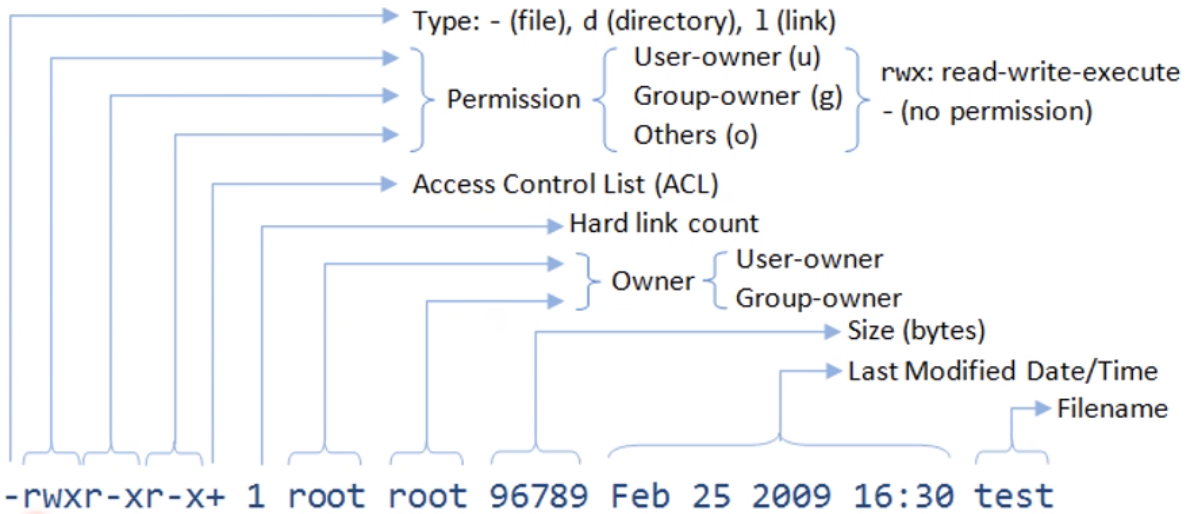
\includegraphics[scale=0.5]{meta}
\end{center}
Schema di output dell'access control list su linux.
La porzione sulle permission è formattata con \emph{rwx} che stanno rispettivamente per \emph{read, write and execute}. Se un valore non è presente vuol dire che quell'utente non ha tale permesso.
\item Mandatory access control (MAC)\\
In questo modello l'accesso è controllato dal sistema operativo o database centralizzato., limitando in base ad un livello gerarchico. Ad ogni utente è assegnato un livello di clearance di sicurezza, e sono in grado di accedere solo ad oggetti di livello minore.
 \item Role based access control\\
In questo modello di accesso i permessi sono attribuiti a ruoli, ed ogni utente si autentica in uno dei ruoli disponibili. Questo modello è particolarmente diffuso in contesti di organizzazioni grandi.
\item Attribute based access control\\
In questo modello di autorizzazione vengono considerate attributi o caratteristiche piuttosto che ruoli per determinare l'accesso. Il controllo è centralizzato, comporta un consistente sforzo computazionale
 \end{itemize}
 
 \emph{Identity, Credential and Access Management}\\
 E' un meccanismo che vuole rimpiazzare i meccanismi di controllo di accessi tradizionali, sviluppato dal governo americano. Una volta completato dovrebbe essere in grado di gestire \textbf{identità digitali}, credenziali, e controllo degli accessi. \\
 
 \emph{Security Audit}\\
La terza parte del golden standard è l'auditing.
L'auditing, che dovrebbe essere un processo indipendente, consiste nel review and examination dei log del sistema per accettarci della qualità ed adeguatezza della security policy aziendale. \emph{L'audit trail} è l'insieme dei dati, o record che vengono salvati durante il processo di auditing. L'auditing può esser fatto per verificare la compliance della security policy, ma anche per verificare l'efficienza dei meccanismi del sistema, l'accesso ad applicazioni selezionate, o i tentativi di accesso remoto.
 \begin{center}
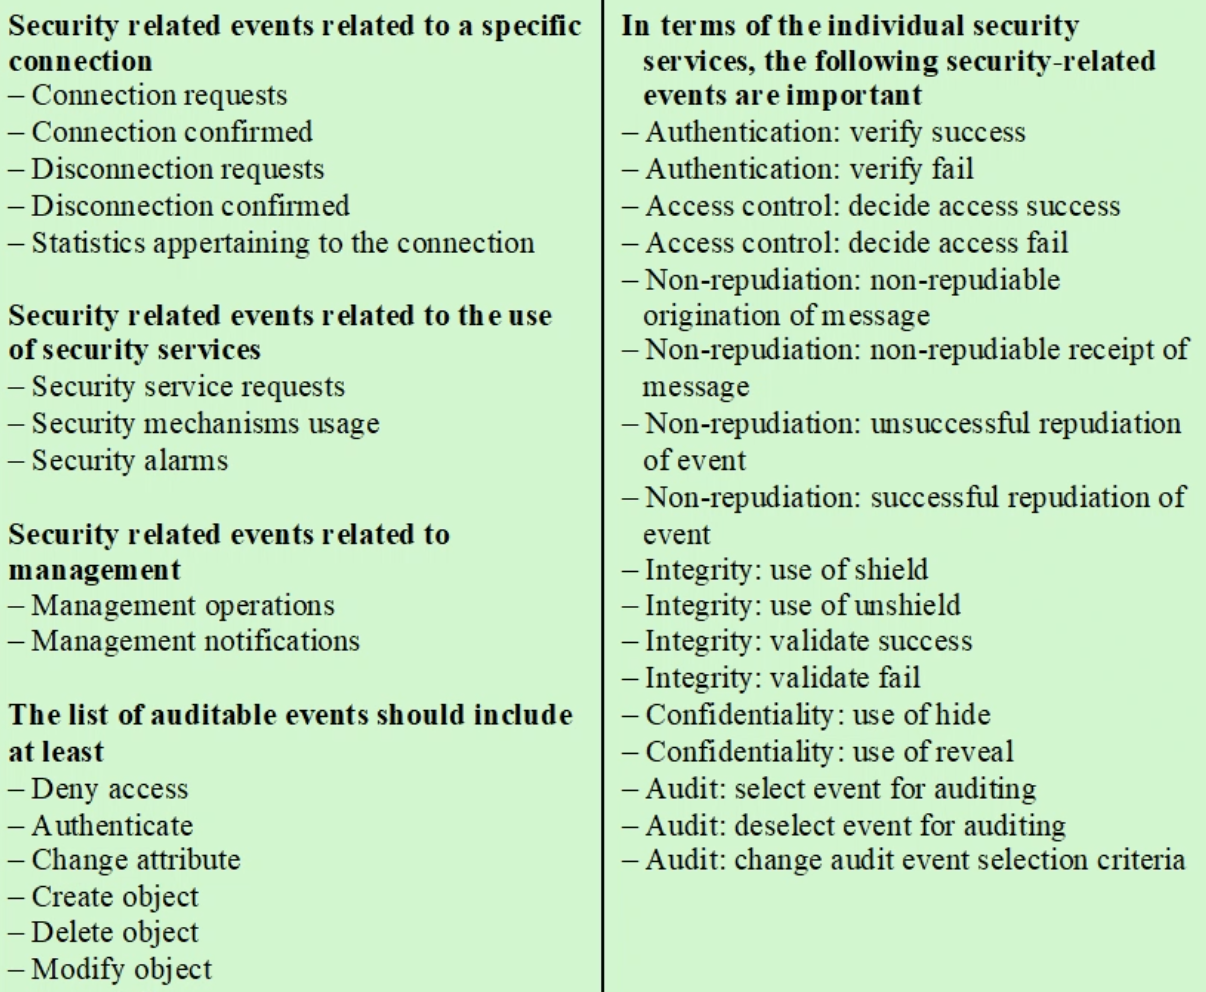
\includegraphics[scale=0.4]{aud}\\
\emph{Standard EU: ISO27002 | NIST}
\end{center}
L'auditing trails possono essere generati anche da accessi fisici, in particolare da system di smartcard, o sistemi d'allarme. Gli audits possono essere registrati:
\begin{itemize}
\item write/read su file sul sistema host: semplice ed efficiente, ma vulnerabile ad accessi da parte dell'attaccante
\item write-only device: stampanti che registrano l'attività, che tuttavia non è pratico per raccogliere una grossa quantità di dati
\item write-once/read many: sistemi su cui i dati una volta scritti non possono essere cancellati (ad esempio DVD)
\end{itemize}
Questi dati possono essere integrati con meccanismi di encryption, digital signature e controllo degli accessi. Una volta raccolti i dati l'analisi viene effettuata per verificare se ci sono violazioni della policy.
La trail analysis possono essere fatte attraverso software dedicato, ad esempio SIEM Systems; è un software centralizzato di logging, complesso ma costoso.\\

 \emph{Computer attacks}\\
 Quando un programma presenta dei bachi, questi possono portare a implicazioni che riguardano la sicurezza. Questi possono portano a problemi di integrità, fino a la possibilità d'esecuzione di codice malevolo.\\
 \emph{Buffer overflow}
  \begin{center}
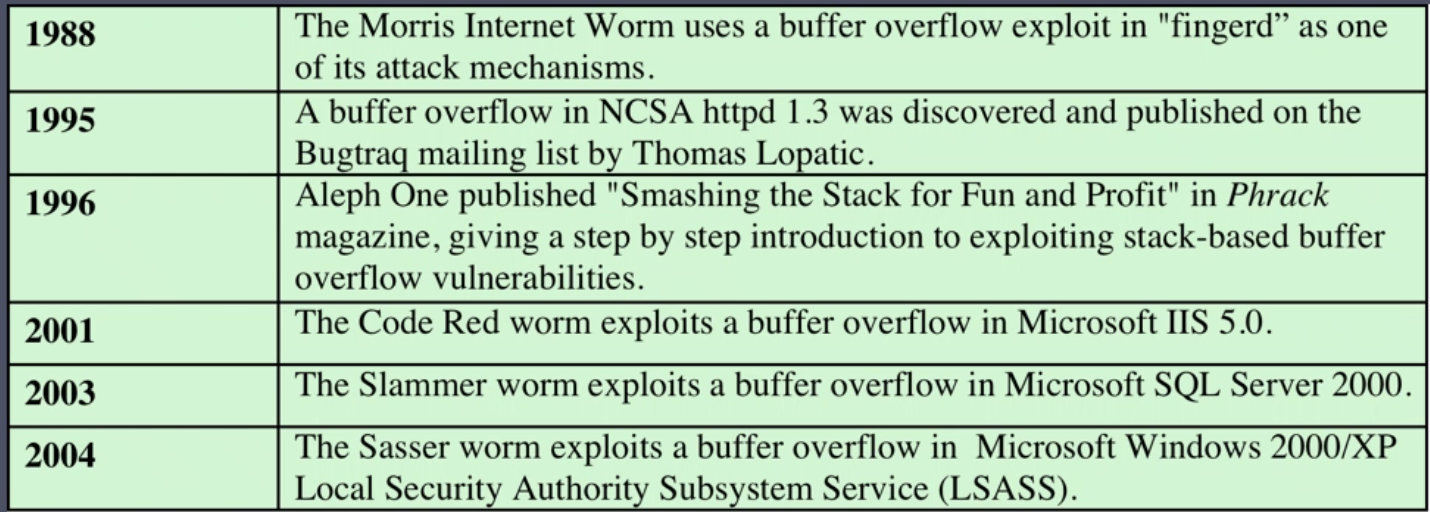
\includegraphics[scale=0.5]{hist}\\
\emph{History of the buffer overflow}
\end{center}
First used by the Morris Worm in 1988, nowadays there are plenty of defence mechanisms known, but it's still a major concern. Buffer overflows exploits take advantage of programming errors. This leaves the possibility by the attacker to escalate permissions.\\
Using tools such as fuzzing attackers can identify potentially vulnerable programs. The shellcode is the code supplied by the attacker, which is saved in the buffer being overflowed. It's specific to processors and operating systems. Metasploit Project provides useful information to people who perform penetration testing. Buffer overflow defenses can be divided into two broad approaches:
\begin{itemize}
\item compile-time defences: through the hardening of programs to resist attacks\\
stack-protection (guard or shield) (canary): viene aggiunto un valore casuale canary non prevedibile, che viene posizionato prima del return address nello stack. Quando il valore risulta modificato sappiamo che c'è stato un attacco.\\
\item run-time defence: through detection and abortion of malicious programs\\
Executable address space protection: lo stack è reso una porzione di memoria non eseguibile. Il problema con questo approccio è che alcune dll sono caricate sullo stack. E' quindi impiegata la MMU per gestire i casi speciali\\
Address space randomization: la posizione degli indirizzi degli stack, heap, global data sono randomizzati.
\end{itemize}
In seguito all'implementazione dello stack non eseguibile è stato formalizzato un nuovo tipo di attacco, ovvero il return to System Call, il flusso del controllo è reindirizzato ad una porzione di codice del sistema operativo che contiene già i comandi per l'esecuzione di una shell
\section*{Malicious Software}
Il malware è un programma caricato in un sistema con l'intento di violare la confidenzialità, integrità dei dati dell'utente di un sistema. Si differenziano principalmente in base a come si diffondono, e a che azioni vengono svolte quando un sistema è infettato.\\
I malware sono principalmente sviluppati da: criminali, crimine organizzato, organizzazioni for profit, agenzie governative, attaccanti politicamente motivati; ma principalmente per soldi\\
I meccanismi di diffusione sono: il malware infetta contenuti all'interno del sistema, per poi diffondersi ad altri sistemi, il alternativa il malware può sfruttare vulnerabilità del sistema per infettare il sistema, per poi replicarsi (in questo caso parliamo di worm), infine casi di social engineering, l'utente è indotto ad abbassare sistemi di sicurezza, e installare trojants.\\
Un tempo per sviluppare un attacco richiedeva la programmazione da parte di programmatori proficient, oggigiorno tuttavia possono essere acquistati toolkits per la generazione di malware, ad esempio Zeus e Angler.\\
\emph{I componenti di un virus}
\begin{itemize}
\item Infection mechanisms, chiamati anche vettori di infezione
\item Trigger, evento o condizione che attiva il payload
\item Payload, l'azione che svolge il virus
\end{itemize}
Il worm è il tipo di virus più importante, è un programma che si diffonde su più macchine, infettandole e ripetendo il processo automaticamente. I worms sfruttano vulnerabilità di sicurezza (nel caso del Morris worm il process fingerd). La diffusione avviene via connessioni di rete, via mail, via file sharing o dispositivi rimovibili. Il worm, a differenza del virus, si diffonde in maniera autonoma.\\
Per diffondersi, il worm utilizza diverse tecniche per irlevare potenziali host target, queste possono essere random (generazione di ip), scanning, hit list (file pregenerato di bersagli), topologici (il worm utilizza informazioni presenti nel sistema per selezionare il prossimo bersaglio), subnet locale.



\subsection*{}




\end{document}  


